\graphicspath{{figures/test/}}

\chapter{Testing}\label{ch:testing} This chapter tests and evaluates whether the system meets the requirements in \autoref{ch:SystemRequirements}. The chapter describes the method of testing each individual requirement and the associated result. In more than one case the product and available testing space limit the tests. In those cases an ideal test is described first followed by the description of the actual test performed.

The ideal accept test should have the transmitter mounted on a drone. The powered-down stand is placed \SI{20}{\meter} away from the drone and would be manually set to point approximately at the drone. The stand is then turned on. The drone should take off and fly around a bit to confirm the operation of the tracking.
This should be followed by a series of tests of the drone moving at top speed around the stand, at a distance between 20 and \SI{120}{\meter}.
Because the oscillators are replaced by large, mains-powered signal generators this test is not an option.

A table of the requirements, results and respective fulfillment is in \autoref{sec:test_results}.

\section{Tests for tracking module}
\textbf{\autoref{req:track_distance}: How far are the receiving antennas able to track the transmitter?}\\
Ideal test: 
This requirement is tested by turning on the transmitter and moving this signal source away until the tracking system is no longer able to detect the \gls{aoa} of the transmitter signal with an angular deviation below \SI{2.08}{\milli\radian}. The tracking system should be pointed directly at the source and the calculated angle is noted and compared to the actual \gls{aoa} at the given distance. The distance is measured using measuring tape. The system should also be able to give a rough estimation of the \gls{aoa} when it is between \SI{-90}{\degree} and \SI{90}{\degree}. \\
Limited test: 
In the final implementation of the system the oscillators have been replaced by signal generators which are not battery powered. Therefore the distance is limited by the length of the available power cords which is \SI{50}{\meter}. 

\textbf{\autoref{req:track_speed}: How fast is the tracking module able to detect a signal?}\\
The time it takes for the tracking system to measure and calculate two angles from three signals which are out of phase at the input ports of the \gls{adc} can be taken to describe whether the tracking system is able to keep track of a drone moving at speeds up to \SI{24.7}{\meter\per\second}. To achieve this tracking speed with a precision better than \SI{2,08}{\milli\radian}, the system should update every \SI{20.2}{\milli\second}, since a target moving at a speed of \SI{24.7}{\meter\per\second} will have moved \SI{50}{\centi\meter} (size specified in \autoref{sec:RequiredPrecision}) in \SI{20.2}{\milli\second} as calculated in \autoref{eq:needed_time}.
\begin{equation} \label{eq:needed_time}
\frac{\SI{0.5}{\meter}}{\SI{24.7}{\meter\per\second}} = \SI{20.2}{\milli\second}
\end{equation}

The tracking system is connected to two signal generators where the phase difference can be controlled representing the IF frequency output from the mixer. The \gls{aoa} is then calculated at different IF frequencies phase differences and the angles are compared and the precision is noted.


\textbf{\autoref{req:track_precision}: How precise is the tracking solution?}\\
Ideal test:
The laser is fitted and attached so it is pointing straight as seen from the antennas and pointed at the transmitter. The tracking system outputs calculated \gls{aoa} of the transmitter which should be zero. This precision is noted and the distance is varied from \SI{20}{\meter} to \SI{120}{\meter} and the test is executed at different angles. The precision is only needed when the antennas are pointing straight at the transmitter therefore only this measurement should be sufficient. \\
Limited test: Because the oscillators are replaced by signal generators the transmitter is only able to move \SI{50}{\meter} from the antenna stand.


\textbf{\autoref{req:track_com}: Can the tracking module communicate its found \gls{aoa} to the mechanical module?} \\
This is tested by having the mechanical module react according to the received angle.

\newpage
\section{Test for mechanical module}
\textbf{\autoref{req:mech_com}: Is the stand able to receive pointing instructions from the tracking module?}\\
Both the stepper and the DC motor are set to move the angle given by the tracking module. The moved angle is noted and compared to the angle given.

\textbf{\autoref{req:mech_laser}: Is the stand able to support a laser?}\\
It is tested if the stand is able to support the laser while it is turning \SI{360}{\degree} clockwise and then counter clockwise in azimuth, and \SI{90}{\degree} up and then down in elevation at full speed without the laser falling off.

\textbf{\autoref{req:mech_precision}: How precise is the stand able to point at a indicated direction?}\\
The stand's pointing precision is tested by a laser attached at the center of the antennas and is set to point at the center of a piece of cardboard. The place where the laser hits is noted and the precision is calculated.

\textbf{\autoref{req:mech_speed}: How fast is the stand able rotate in azimuth and elevation direction?}\\
The speed of the stand in azimuth direction is tested by applying the maximum output voltage of the DC motor driver, directly to the DC motor and measuring the rotational speed. 
The stepper motor is tested with the \SI{200}{\hertz} stepping frequency as described in \autoref{sec:stepperMotor}. 

\newpage
\section{Requirement results} \label{sec:test_results}
\begin{table}[h]
	\centering
	\caption{Test results of the tracking module requirements. Results that are partially satisfied are enclosed in parenthesis.} \label{tab:ResultTR}
	\begin{tabularx}{\textwidth}{l X X c}
		\textit{ID}		&	\textit{Description} &\textit{Results} &\textit{Accepted} \\ \rowcolor{lightGrey} \toprule
TR1 & The tracking module should be able to detect the drone at distances of up to \SI{120}{\meter}. & Only tested at a distance up to \SI{41}{\meter} which resulted in a precision worse than \SI{2.08}{\milli\radian}. The \gls{aoa} is still estimated, but the field of view is from \SI{-40}{\degree} to \SI{45}{\degree} in the azimuth direction and \SI{-45}{\degree} to \SI{45}{\degree} in elevation direction. & (Yes) \\
TR2 & The tracking module should be able to keep track of a drone moving at speeds up to \SI{24,7}{\meter\per\second}. & The time it takes to estimate the \gls{aoa} is \SI{46}{\milli\second} and it should be below \SI{20.2}{\milli\second} to keep track of a drone moving \SI{24.7}{\meter\per\second}. & No \\ \rowcolor{lightGrey}
TR3 & The tracking module must be able to locate the drone with a maximum angular deviation of \SI{2,08}{\milli\radian}. & The tracking solution can estimate an angle from two out of phase sinusoids with a deviation of \SI{1.89}{\milli\radian}. The complete tracking solution estimates the \gls{aoa} when directly pointed at the transmitter with a precision of \SI{25.6}{\milli\radian} at a distance of \SI{21}{\meter}. & No \\ 
TR4 & The tracking module should be able to communicate the found angles to the mechanical module. & The antenna stand is moved whenever the found \gls{aoa} is changed. & Yes \\ 
	\end{tabularx}
\end{table}

\begin{table}[h]
	\centering
	\caption{Test results of the mechanical module requirements.}
	\label{tab:ResultMECH}
	\begin{tabularx}{\textwidth}{l X X c}
		\textbf{ID}		&	\textbf{Description} &\textbf{Results} &\textbf{Accepted} \\ \rowcolor{lightGrey} \toprule
MECH1 & The stand should be able to receive pointing instructions from the tracking module. & DC-motor rotates the right direction depending on the received pointing instructions and the stepper motor rotates a given angle with a deviation up to \SI{16}{\percent}. Because of the feedback loop in the controller, it rotates until the phase difference is \SI{0}{\degree}. & Yes \\
MECH2 & The stand must be able to support a laser. & The stand is able to support a laser. & Yes \\ \rowcolor{lightGrey}
MECH3 & The stand must point in the indicated direction with a maximum angular deviation of less than $\pm$\SI{2.6}{\milli\radian} in azimuth and less than $\pm$\SI{2.6}{\milli\radian} in the elevation angel. & As described in \autoref{ch:MechanicalModels}. & No \\
MECH4 & The stand should be able to rotate with an angular velocity of up to \SI{1.236}{\radian\per\second} in the azimuth direction and \SI{1.236}{\radian\per\second} in the elevation direction. & The stand is able to rotate with an angular velocity of \SI{2.666}{\radian\per\second} in the azimuth direction and \SI{0,518}{\radian\per\second} in the elevation direction.  & No \\ 
	\end{tabularx}
\end{table}

\begin{table}[h]
	\centering
	\caption{Test results of the compatibility requirements.}
	\label{tab:ResultCOMP}
	\begin{tabularx}{\textwidth}{l X X c}
		\textbf{ID}		&	\textbf{Description} &\textbf{Results} &\textbf{Accepted} \\ \rowcolor{lightGrey} \toprule
COMP1 & The entire design should be implemented to fit on the motorized antenna stand. & Everything designed to fit on the antenna stands fits but because the oscillators have been replaced by signal generators it no longer fits. & No \\
COMP2 & The design should not expose the motors to voltages above their maximum operational values. & Motors are not exposed to more than \SI{10}{\volt} which is below the rated maximum operational value & Yes
	\end{tabularx}
\end{table} 
\clearpage


\section{Accept test}
Ideal test: 
The transmitter is attached centrally on the underside of drone. The drone carries a \SI{50x50}{\centi\meter} grid of solar panels and a system to detect which one of the panels is hit. Which panel is hit is used to estimate the precision of the pointing, and the information is communicated down to the ground in real time. The drone is flown at different speeds, directions and distances and the error in tracking is compared.
The precision is noted at distances from \SI{20}{\meter} to \SI{120}{\meter} and the speed of the drone should be varied between zero and \SI{24.7}{\meter\per\second}. \\
Limited test:
Because the oscillators are replaced by large signal generators the transmitter cannot be mounted on the drone. 
The transmitter connected to a signal generator is placed on a trolley and a power extension cord is used to supply the generator with mains power. For the testing \SI{50}{\meter} of extension cord is available, limiting the distance between the transmitter and the receiver. The trolley makes the transmitter movable but the speed is very limited compared to a drone. The trolley with the transmitter is placed at a distance of \SI{21}{\meter} and driven back and forth on a straight pathway to test the tracking in the azimuth direction. The elevation test is done by changing the inclination of the antenna stand using standoffs.

On \autoref{fig:accept_test_img} the test setup is seen where the laser dot hits the transmitter antenna with a precision of \SI{1.9}{\milli\radian} at a distance of \SI{21}{\meter}. At this distance the laser dot hit the center of the box within \SI{4}{\centi\meter}.
This gives an angular precision of \SI{1.9}{\milli\radian} as calculated in \autoref{eq:accept_test_precision}.
\begin{equation} \label{eq:accept_test_precision}
\theta = \arctan\left(\frac{\SI{4}{\centi\meter}}{\SI{21}{\meter}}\right) = \SI{1.9}{\milli\radian}
\end{equation}

\begin{figure} [h]
\centering
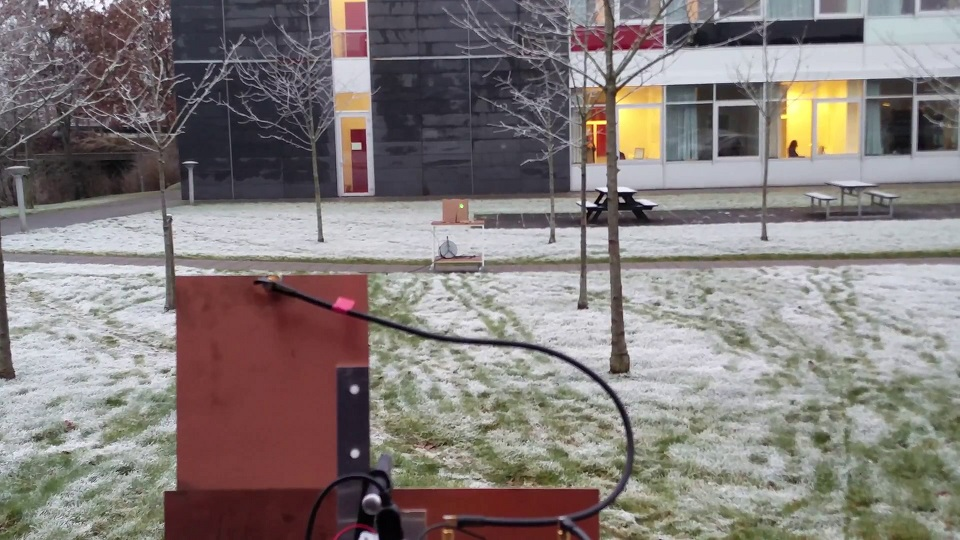
\includegraphics[width=0.6\linewidth]{accept_test_img}
\caption{Image showing the setup of the accept test where the laser dots hits cardboard box behind the transmitting antenna.}
\label{fig:accept_test_img}
\end{figure}
At a distance of \SI{41}{\meter} the system is not able to point at the transmitter within \SI{2.08}{\milli\radian}. 
When moving the transmitter the laser dot follows the transmitter at \SI{21}{\meter} and \SI{41}{\meter} but in azimuth direction the movement is jerky. A large overshoot is observed in this direction which means it takes a while for it to settle.
